%TODO: ARREGLAR EJERCICIO 1B
\documentclass{article}
\usepackage[utf8]{inputenc}
\usepackage[spanish]{babel}
\usepackage{graphicx, graphics, float, hyperref}
\usepackage{listings}
\usepackage[a4paper, total={6in, 10in}]{geometry}

\title{SSO Práctica 1 Sesión 2}
\author{Andrés Merlo Trujillo}
\date{}
\hypersetup{
    colorlinks=true,
    linkcolor=black,
}

\begin{document}

\maketitle

\tableofcontents

\newpage
\addcontentsline{toc}{section}{Ejercicio 1}
\section*{Ejercicio 1}

\addcontentsline{toc}{subsection}{Apartado A}
\subsection*{Apartado A}
Mediante la orden \verb|lsof -i| ejecutada como root, podemos obtener la informacion de los servicios y procesos que tienen alguna conexion abierta o archivo abierto.

%foto de lsof -i

La orden ofrece 9 columnas con los siguientes signifiacdos:

\begin{itemize}
    \item \textbf{COMMAND: }Nombre del comando asociado al proceso/archivo.
    \item \textbf{PID: }Process IDentificator (identificador de proceso).
    \item \textbf{USER: }UID del usuario al que pertenece el proceso/archivo.
    \item \textbf{FD: }Descriptor de fichero.
    \item \textbf{TYPE: }Tipo de archivo asociado al mismo (GDIR, GREG, ...) o indica el tipo de conexion (en cpaa de red) (IPv4, IPv6, X.25, etc.).
    \item \textbf{DEVICE: }Numero de dispotivio.
    \item \textbf{SIZE/OFF: }Tamaño del archivo.
    \item \textbf{NODE: }Numero de nodo/inodo de un fichero o el procotolo en capa de transporte (TCP, UDP, ...).
    \item \textbf{NAME: }Punto de montaje y sistema de archivos que usa el archivo abierto. Tambien puede significar la direccion local o remota de internet o de un socket.
\end{itemize}

A continuación explicaré dos procesos de la salida del comando anterior:

\addcontentsline{toc}{subsubsection}{sshd}
\subsubsection*{sshd}
\begin{itemize}
    \item \textbf{COMMAND: }sshd
    \item \textbf{PID: }1319
    \item \textbf{USER: }root
    \item \textbf{FD: }3u/4u (FDs 3 y 4. La letra ``u'' indica acceso de lectura y escritua)
    \item \textbf{TYPE: }IPv4/IPv6 (está a la espera de recibir algo en las dos versiones del protocolo IP.)
    \item \textbf{DEVICE: }22997/23008
    \item \textbf{SIZE/OFF: }0t0 (Offset, el segundo ``0'' indica que no hay offset)
    \item \textbf{NODE: }TCP (usan este protocolo de transporte porque asegura que se reciben los paquetes mediante ACKs).
    \item \textbf{NAME: }*:ssh (LISTEN) (El asterisco indica que espera de cualquier IP, en el puerto ssh (configurable, por defecto el 22)).
\end{itemize}

\addcontentsline{toc}{subsubsection}{avahi-daemon}
\subsubsection*{avahi-daemon}
\begin{itemize}
    \item \textbf{COMMAND: }avahi-dae (avahi-daemon)
    \item \textbf{PID: }1144
    \item \textbf{USER: }avahi
    \item \textbf{FD: }14u (FD 14. La letra ``u'' indica acceso de lectura y escritua)
    \item \textbf{TYPE: }IPv6
    \item \textbf{DEVICE: }22668
    \item \textbf{SIZE/OFF: }0t0 (Offset, el segundo ``0'' indica que no hay offset)
    \item \textbf{NODE: }UDP
    \item \textbf{NAME: }*:53167 (Cualquier IP en el puerto 53167).
\end{itemize}


\addcontentsline{toc}{subsection}{Apartado B}
\subsection*{Apartado B}
Leyendo el manual, hace falta usar el switch ``-i'', como en el apartado anterior, y añadiendo que busque las conexiones con el servicio ``ssh''. Por tanto, el comando quedaria asi: \verb|lsof -i :ssh|.

%foto del comando sin ssh desde host

Ahora mismo no hay nadie conectado, solo estan los ``daemons'' a la escucha de peticiones de conexion. Si ahora me conecto desde el otra maquina virtual a la de Ubuntu, la salida es la siguiente:

%foto del comando con ssh desde host.

Aparecen dos lineas nuevas y en el apartado \verb|NAME| se ve que la conexion es entre el usuario ``andres-kvm'' (Ubuntu) usando el servicio ``ssh'' (en mi caso es el puerto 22)  y el usuario ``archlinux'' en el puerto 57686, que es un puerto que se asigna aleatoriamente para enviar informacion (escuchar) a ``archlinux''.

Con la orden \verb|lsof -c sshd| se puede ver los archivos que tiene abiertos SSH:

%foto de alguno importante

Como se puede ver, aparece el usuario conectado y con el mismo PID aparecen todos los archivos abiertos por \verb|sshd|


\addcontentsline{toc}{subsection}{Apartado C}
\subsection*{Apartado C}
Para mostrar los archivos que usa un proceso concreto, es necesario referenciarlo con su PID. Para ello es necesario usar el siguiente comando: \verb|lsof -p PID|.

%foto de lsof -p 

Y ahora para ver los archivos que esta usando un usuario concreto, se debe usar el switch ``-u'': \verb|lsof -u usuario|

%foto de lsof -u
%caption: salida de lsof -u andres, se puede ver que en la tercera columna solo aparece ese usuario.

Por ultimo, para obtener los archivos que tiene abiertos un proceso \textbf{Y} un usuario, es necesario usar el switch adicional ``-a''. Esto es debido a que por defecto solo busca, en caso de haber varios switches, utilizando un criterio \textbf{OR}. Comando: \verb|lsof -u usuario -p PID -a|

%img de eso
%caption: archivos aboiertps por el PID PID y el usuario root

\addcontentsline{toc}{section}{Ejercicio 2}
\section*{Ejercicio 2}
\addcontentsline{toc}{subsection}{Apartado A}
\subsection*{Apartado A}
Para ver que vulnerabilidades hay en el sistema es neceasrio instalar el paquete \verb|lynis| junto al comando \verb|lynis audit system|.

%foto de los resultados

Y las posibles vulnerabilidades son las siguientes:

%foto de los warnings

Como se puede ver, solo hay dos avisos. Suponiendo que es una maquina para desarrollar aplicaciones, voy a listar los grados de severidad:

\begin{itemize}
    \item \textbf{Found one or more vulnerable packages. [PKGS-7392]} $\rightarrow$ Severidad: \textbf{Alta}. Puede llegar a ser muy peligroso, ya que pueden ser vulnerabilidades que potencialmente le otorguen acceso root al sistema. 
    
    \textbf{Solucion: }Para solucionarlo, es necesario actualizar todos los paquetes del sistema con la orden (en Ubuntu y en distros basadas en Debian) \verb|sudo apt upgrade|.


    \item \textbf{iptables module(s) loaded, but no rules active [FIRE-4512]} $\rightarrow$ Severidad: \textbf{Alta}. \verb|iptables| es un paquete que se utiliza principalmente junto a un firewall para permitir/bloquear cierto trafico. Si fuera una compañia importante sin firewall, podria darse el caso de que alguien entrase en el sistema y obtuviese datos sin permiso, produciendo asi un ``leak'' o incluso chantaje.
    
    \textbf{Solucion: }La solucion es habilitar el firewall y aplicarle las reglas que sean necesarias. En Ubuntu viene instalado por defecto \verb|ufw|, pero viene deshabilitado por defecto. Para habilitarlo hay que poner: \verb|sudo ufw enable| y con la orden \verb|sudo ufw status verbose| se pueden ver las reglas (por defecto prohibe trafico entrante y permite trafico saliente, prohibiendo asi conexiones del tipo SSH).

    %foto del status
\end{itemize}

Ahora, ejecutando de nuevo \verb|lynis audit system| aparece la siguiente puntuacion:

%puntuacion nueva (mas alta)

Y al ver los warnings se ve que no aparece ninguno:

%foto de great, no warnings

Por tanto, a nivel de advertencias el sistema ya está ``seguro'' (nunca se puede decir con seguridad). En cuanto a las sugerencias, las principales son para reforzar SSH y el uso de bloqueadores de IP como ``fail2ban''. No son fallos demasiado críticos.

\addcontentsline{toc}{subsection}{Apartado B MAL}
\subsection*{Apartado B MAL}
Con el comando \verb|lynis show tests| podemos obtener todos los tests que realiza:

%comando lynis show tests

Y se puede ver que el codigo de uno de ellos es ``MALW-*''

%comando resaltando el test
%caption: El test MALW-3280 es el que me interesa
Ahroa con el comando \verb|lynis show details MALW-3280|
%foto 1
%foto 2

Por tanto, la lista de antivirus que escanea son: Avast, Avira, epagd, CrowdStrike, CylanceSvc, esets\_daemon, Kapersky, McAffee, savscand, SophosScanD, rtvscand, Symantec management client service, Symantec Endpoint Protection configuration service, synoavd, Trend Micro Deep Anti Malware component y TmccMac to test for Trend Micro anti-virus (macOS)

Además, con la orden \verb|lynis show tests| también aparecen en la seccion ``MALW'' algunos antivirus extras, estos son: ClamAV, Rootkit Hunter, LMD y chkrootkit

%foto de la lista resaltada


Ahora instalaré ``unhide'' con la orden \verb|sudo apt install unhide|. Una vez hecho esto, seguirá saliendo en el report que no tengo antivirus.

%foto de lo ocurrido con unhide que no sale

\addcontentsline{toc}{subsection}{Apartado B}
\subsection*{Apartado B}
Lynis permite añadir nuevos tests o modificar existentes para añadirles más funcionalidad. Todo esto se realiza mediante los archivos que se encuentran en el directorio \verb|/usr/share/lynis/include|.

En este caso, para poder ver los antivirus que detecta actualmente es necesario inspeccionar el archivo \verb|/usr/share/lynis/include/tests_malware|:

%fotos del contenido de este archivo (incluyendo algun codigo con el comentario del antivirus)

Como se puede ver, detecta los siguientes antivirus: 

\begin{itemize}
    \item Avast
    \item Avira
    \item Bitdefender
    \item ClamAV (clamd, clamscan y freshclam)
    \item CrowdStrike
    \item ESET
    \item Kapersky
    \item McAffee
    \item chkrootkit
    \item rkhunter
    \item LMD
    \item CylanceSvc
    \item SophosScanD
    \item Symantec
    \item Synology Antivirus Essential
    \item Trend Micro Anti Malware for Linux
\end{itemize}

Ahora voy a instalar el programa ``unhide'', el cual no es detectado por Lynis:

%foto de que no encuetra antivirus

AHora, modifico el archivo anterior y añado la macro:

%foto con la nueva macro

Y añadimos un nuvo ``if'' en la cadena de ``if'' del test ``MALW-3280'':

%foto de ese if resaltado

Y ahora al pasar el test ya aparece como que existe un antivirus:

%foto del test OK en malware scanner

Y si desinstalo \verb|unhide| aparece como que no hay ningún antivirus instalado:

%foto del test no OK en malware scanner


\addcontentsline{toc}{section}{Ejercicio 3}
\subsection*{Ejercicio 3}

Para instalar la herramienta en Ubuntu se ejecuta la orden: \verb|sudo apt install rkhunter|.

\addcontentsline{toc}{subsection}{Apartado A}
\subsection*{Apartado A}
Para realizar el analisis es necesario ejecutar el comando: \verb|sudo rkhunter --check|

%foto de la salida de rkhunter

Como se puede ver en los resultados, aparece que hay alguna advertencia. Ahora, revisando el archivo \verb|/var/log/rkhunter.log| y buscando la palabra ``Warning''.

%foto de los warnings

La primera advertencia tiene que ver con la posible modificacion del binario \verb|lwp-request|, ne caso de ser una modificacion malintencionada, un atacante podria modificar el binario para recibir todos los datos que se envian o reciben a traves de el (por ejemplo, si se usa SSH, poner un keylogger para obtener las contraseñas).

%foto
El segundo error tiene que ver con la seguridad de la configuracion SSH, ya que el parametro ``PermitRootLogin'' no esta puesto a ninugn valro y por defecto puede ser ``Yes'', dando la posibilidad de que un atacante pueda a entrar al sistema por SSH como usuario root.


\addcontentsline{toc}{subsection}{Apartado B}
\subsection*{Apartado B}
El primer error se puedde solucionar cambiando en \verb|/etc/rkhunter.log| el macro \verb|PKGMGR| (por defecto esta a ``NONE''), en el caso de Ubuntu y Debian se debe cambiar a ``DPKG''. Este cambio hace que coteje con los hashes de cada paquete para ver si ha sido modificado malintencionadamente:

%Foto de la macro cambiada

Una vez realizado este cambio, se debe ejecutar el comando \verb|sudo rkhunter --propupd|.


Todo esto se puede solucionar cambiando en el archivo de configuracion \verb|/etc/ssh/sshd_config| y poniendo el parametro a ``no'':

%foto del cambio

Ademas, es necesario reinicar el servicio con el comando \verb|systemctl restart ssh|.

Por ultimo, para comprobar que el sistema ya no tiene mas advertencias, ejcutamos de nuevo la orden \verb|sudo rkhunter --check|:

%foto del resumen de warnings

Y como se puede ver, le sistema ya es seguro, eran solo falsos positivos en el primer caso, y en el segundo una mala configuracion de un servicio importante.


\end{document}

%\begin{figure}[H]
%    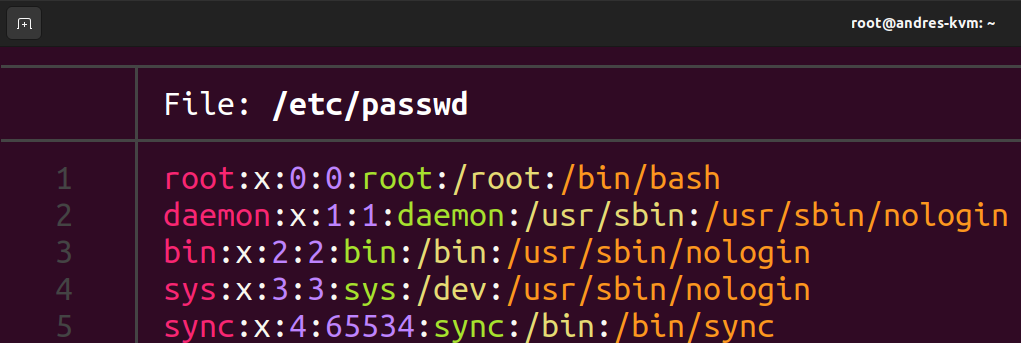
\includegraphics[width=\textwidth]{imagenes/passwdfile.png}
%    \caption{Ejemplo de entradas en el archivo.}
%\end{figure}